% The bibliography travels inside this file: LaTeX writes smartlocker-refs.bib at compile time,
% so no separate .bib has to be uploaded (it is overwritten on every run).
\begin{filecontents*}[overwrite]{smartlocker-refs.bib}
@article{alfuqaha2015iot,
  author  = {Al-Fuqaha, Ala and Guizani, Mohsen and Mohammadi, Mehdi and Aledhari, Mohammed and Ayyash, Moussa},
  title   = {Internet of Things: A Survey on Enabling Technologies, Protocols, and Applications},
  journal = {IEEE Communications Surveys \& Tutorials},
  volume  = {17},
  number  = {4},
  pages   = {2347--2376},
  year    = {2015}
}

@article{sicari2015security,
  author  = {Sicari, Sabrina and Rizzardi, Alessandra and Grieco, Luigi Alfredo and Coen-Porisini, Alberto},
  title   = {Security, Privacy and Trust in {Internet of Things}: The Road Ahead},
  journal = {Computer Networks},
  volume  = {76},
  pages   = {146--164},
  year    = {2015}
}

@article{iwan2016parcel,
  author  = {Iwan, Stanis{\l}aw and Kijewska, Kinga and Lemke, Justyna},
  title   = {Analysis of Parcel Lockers' Efficiency as the Last Mile Delivery Solution -- The Results of the Research in {Poland}},
  journal = {Transportation Research Procedia},
  volume  = {12},
  pages   = {644--655},
  year    = {2016}
}

@article{mitrokotsa2010rfid,
  author  = {Mitrokotsa, Aikaterini and Rieback, Melanie R. and Tanenbaum, Andrew S.},
  title   = {Classifying {RFID} Attacks and Defenses},
  journal = {Information Systems Frontiers},
  volume  = {12},
  number  = {5},
  pages   = {491--505},
  year    = {2010}
}

@article{chandola2009anomaly,
  author  = {Chandola, Varun and Banerjee, Arindam and Kumar, Vipin},
  title   = {Anomaly Detection: A Survey},
  journal = {ACM Computing Surveys},
  volume  = {41},
  number  = {3},
  pages   = {15:1--15:58},
  year    = {2009}
}

@inproceedings{sommer2010outside,
  author    = {Sommer, Robin and Paxson, Vern},
  title     = {Outside the Closed World: On Using Machine Learning for Network Intrusion Detection},
  booktitle = {Proc. IEEE Symposium on Security and Privacy},
  pages     = {305--316},
  year      = {2010}
}

@article{moustafa2021toniot,
  author  = {Moustafa, Nour},
  title   = {A New Distributed Architecture for Evaluating {AI}-Based Security Systems at the Edge: Network {TON\_IoT} Datasets},
  journal = {Sustainable Cities and Society},
  volume  = {72},
  pages   = {102994},
  year    = {2021}
}

@article{hall2009weka,
  author  = {Hall, Mark and Frank, Eibe and Holmes, Geoffrey and Pfahringer, Bernhard and Reutemann, Peter and Witten, Ian H.},
  title   = {The {WEKA} Data Mining Software: An Update},
  journal = {ACM SIGKDD Explorations Newsletter},
  volume  = {11},
  number  = {1},
  pages   = {10--18},
  year    = {2009}
}

@article{breiman2001rf,
  author  = {Breiman, Leo},
  title   = {Random Forests},
  journal = {Machine Learning},
  volume  = {45},
  number  = {1},
  pages   = {5--32},
  year    = {2001}
}

@book{quinlan1993c45,
  author    = {Quinlan, J. Ross},
  title     = {C4.5: Programs for Machine Learning},
  publisher = {Morgan Kaufmann},
  address   = {San Mateo, CA},
  year      = {1993}
}

@inproceedings{john1995nb,
  author    = {John, George H. and Langley, Pat},
  title     = {Estimating Continuous Distributions in {Bayesian} Classifiers},
  booktitle = {Proc. 11th Conference on Uncertainty in Artificial Intelligence (UAI)},
  pages     = {338--345},
  year      = {1995}
}

@article{aha1991ibl,
  author  = {Aha, David W. and Kibler, Dennis and Albert, Marc K.},
  title   = {Instance-Based Learning Algorithms},
  journal = {Machine Learning},
  volume  = {6},
  number  = {1},
  pages   = {37--66},
  year    = {1991}
}

@inproceedings{kohavi1995cv,
  author    = {Kohavi, Ron},
  title     = {A Study of Cross-Validation and Bootstrap for Accuracy Estimation and Model Selection},
  booktitle = {Proc. 14th International Joint Conference on Artificial Intelligence (IJCAI)},
  pages     = {1137--1145},
  year      = {1995}
}

@article{haber1991timestamp,
  author  = {Haber, Stuart and Stornetta, W. Scott},
  title   = {How to Time-Stamp a Digital Document},
  journal = {Journal of Cryptology},
  volume  = {3},
  number  = {2},
  pages   = {99--111},
  year    = {1991}
}

@inproceedings{provos1999bcrypt,
  author    = {Provos, Niels and Mazi{\`e}res, David},
  title     = {A Future-Adaptable Password Scheme},
  booktitle = {Proc. USENIX Annual Technical Conference, FREENIX Track},
  pages     = {81--91},
  year      = {1999}
}

@inproceedings{rfidiot2023locker,
  author    = {Bharatiraja, C. and Chittoor, Prithvi Krishna and Bhargava, Yash Vardhan},
  title     = {An {IoT} Based Centralized Smart Locker Using {RFID} Technology},
  booktitle = {AIP Conference Proceedings},
  volume    = {2427},
  number    = {1},
  pages     = {020098},
  publisher = {AIP},
  month     = feb,
  year      = {2023},
  doi       = {10.1063/5.0101139}
}

@article{roman2013features,
  author  = {Roman, Rodrigo and Zhou, Jianying and Lopez, Javier},
  title   = {On the Features and Challenges of Security and Privacy in Distributed {Internet of Things}},
  journal = {Computer Networks},
  volume  = {57},
  number  = {10},
  pages   = {2266--2279},
  year    = {2013}
}

@article{abomhara2015cyber,
  author  = {Abomhara, Mohamed and K{\o}ien, Geir M.},
  title   = {Cyber Security and the {Internet of Things}: Vulnerabilities, Threats, Intruders and Attacks},
  journal = {Journal of Cyber Security and Mobility},
  volume  = {4},
  number  = {1},
  pages   = {65--88},
  year    = {2015}
}

@article{want2006rfid,
  author  = {Want, Roy},
  title   = {An Introduction to {RFID} Technology},
  journal = {IEEE Pervasive Computing},
  volume  = {5},
  number  = {1},
  pages   = {25--33},
  year    = {2006}
}

@article{coskun2013nfc,
  author  = {Coskun, Vedat and Ozdenizci, Busra and Ok, Kerem},
  title   = {A Survey on Near Field Communication ({NFC}) Technology},
  journal = {Wireless Personal Communications},
  volume  = {71},
  number  = {3},
  pages   = {2259--2294},
  year    = {2013}
}

@article{jain2004biometric,
  author  = {Jain, Anil K. and Ross, Arun and Prabhakar, Salil},
  title   = {An Introduction to Biometric Recognition},
  journal = {IEEE Transactions on Circuits and Systems for Video Technology},
  volume  = {14},
  number  = {1},
  pages   = {4--20},
  year    = {2004}
}

@article{ahmed2016survey,
  author  = {Ahmed, Mohiuddin and Mahmood, Abdun Naser and Hu, Jiankun},
  title   = {A Survey of Network Anomaly Detection Techniques},
  journal = {Journal of Network and Computer Applications},
  volume  = {60},
  pages   = {19--31},
  year    = {2016}
}
\end{filecontents*}

\documentclass[journal,onecolumn]{IEEEtran}
\usepackage{cite}
\usepackage{amsmath,amssymb,amsfonts}
\usepackage{graphicx}
\usepackage{textcomp}
\usepackage{float}
\usepackage{tikz}
\usetikzlibrary{arrows.meta,positioning,fit,shapes.geometric}
\tikzset{every picture/.style={line width=0.6pt}}
% pack figures and tables tightly (the paper has many floats)
\renewcommand{\topfraction}{0.9}
\renewcommand{\bottomfraction}{0.8}
\renewcommand{\textfraction}{0.07}
\renewcommand{\floatpagefraction}{0.85}
\setcounter{topnumber}{3}
\setcounter{bottomnumber}{2}
\setcounter{totalnumber}{5}
\setlength{\textfloatsep}{10pt plus 2pt minus 2pt}
\setlength{\floatsep}{8pt plus 2pt minus 2pt}
\setlength{\intextsep}{8pt plus 2pt minus 2pt}

\begin{document}

\title{Smart Locker with Anomalous Access Detection Based on IoT Device Telemetry}

% Every author with the e-mail address under the name; the corresponding author is marked with *.
\author{%
\begin{tabular}{ccc}
Duc Hoang Nguyen & Viet Tien Nguyen & Huy Hoang Nguyen \\
{\small duchoang.nguyen103@gmail.com} & {\small tiennguyen100306@gmail.com} & {\small huyhoang.ct06@gmail.com} \\[8pt]
Thanh Cao Nguyen & Thu Le & Kieu Trong Khanh$^{*}$ \\
{\small thanhcao19112006@gmail.com} & {\small thulvm@fpt.edu.vn} & {\small khanhkt@fpt.edu.vn} \\[8pt]
\multicolumn{3}{c}{FPT University, Ho Chi Minh Campus, Vietnam} \\[2pt]
\multicolumn{3}{c}{\small $^{*}$Corresponding author (ORCID: 0000-0000-0000-0000)}
\end{tabular}}

\maketitle

\begin{abstract}
Shared lockers on university campuses are still opened with mechanical keys or paper codes, cannot be reserved,
and give staff no view of forced doors, lost cards or forgotten items; once networked, their unlock signal can also be
forged or replayed. This paper presents SmartLocker, a locker rental system in which users reserve a slot on a web map,
pay from a prepaid wallet and open it with a personal identification number (PIN), a radio-frequency identification
(RFID) card, a fingerprint or a phone page. The ESP32 box takes no access decision: it forwards every credential to the
server, which replies \texttt{UNLOCK} or \texttt{DENY}. Abnormal access is detected in two tiers: a priority-ordered
rule engine over device telemetry and server context recognises sensor faults, spoofed remote opens, lost cards, forced
opening, wrong-user access, items left behind and overdue storage, and a machine-learning risk score raises an alert
only for sessions that no rule explains. On 480 synthetic labelled sessions, k-nearest neighbours was the best of four
Weka classifiers (weighted F1 of 0.977 in 10-fold cross-validation); its remaining errors lie between wrong-user and
normal sessions, which share the same telemetry by construction, and this supports checking identity by rule. The
system passed 66 unit and integration tests and 472 API assertions in 18 scenarios, six replayed detection scenarios
gave the expected labels, and the server answered device requests in a mean of 6--31~ms per endpoint.
\end{abstract}

\begin{IEEEkeywords}
Smart locker, Internet of Things, ESP32, RFID, anomaly detection, rule engine, machine learning, Weka.
\end{IEEEkeywords}

\section{Introduction}

\IEEEPARstart{S}{elf-service} lockers are now common for parcels and short-term storage in campuses, canteens, gyms
and libraries \cite{iwan2016parcel}. Most of the lockers found on campuses, however, are purely mechanical: a key or a
code on paper opens the door, a slot cannot be booked before the user arrives, and the operator has no record of what
happens at the box. A forced door, a lost card picked up by someone else or belongings left for several days are
discovered only when somebody reports them. The Internet of Things (IoT) \cite{alfuqaha2015iot} makes the state of
every slot visible to a server, but it also brings the classic weaknesses of connected devices: a box can be
impersonated, an unlock message can be forged or replayed, and sensor readings can be wrong or manipulated
\cite{sicari2015security, roman2013features}.

This work addresses both the service and the security side of a shared campus locker. Its guiding principle is that
the box is a thin, authenticated client and that every decision is taken by the server, where the full context of a
booking is available. The main contributions are as follows.
\begin{enumerate}
  \item A complete locker rental system with reservation on a map, prepaid payment, four opening methods (PIN, RFID
        card, fingerprint and phone) and an ESP32 box that only forwards credentials signed with a per-device key; all
        money and time rules run in database transactions.
  \item A two-tier detector of anomalous access, a priority-ordered rule engine followed by a machine-learning risk
        score, complemented by server-side safeguards and a hash-chained audit log.
  \item An evaluation with automated tests, replayed detection scenarios, server response times and four classifiers,
        showing on synthetic data that telemetry alone cannot separate wrong-user from normal access.
\end{enumerate}
Section~II reviews related work. Section~III describes the system design, Section~IV the detection method and
Section~V the implementation. Section~VI reports the evaluation and Section~VII concludes the paper.

\section{Related Work}

\textit{Smart and parcel lockers.} Research on parcel lockers has concentrated on last-mile logistics, where lockers
reduce failed deliveries and courier trips \cite{iwan2016parcel}, rather than on access security. An IoT locker based
on RFID \cite{rfidiot2023locker} identifies the user with an identity card and uses Wi-Fi to monitor the locker, log
accesses and watch for unauthorised use. SmartLocker adds reservation on a map, prepaid payment, several credentials
and a detector that raises typed alerts instead of only recording accesses.

\textit{Security of IoT devices and credentials.} Surveys of IoT security list impersonation, message spoofing and
physical tampering among the main threats to constrained devices \cite{abomhara2015cyber} and recommend that trust be
established on the server side \cite{sicari2015security}. RFID \cite{want2006rfid} is exposed to cloning, replay and
relay attacks \cite{mitrokotsa2010rfid}, and near field communication (NFC) readers inherit these risks
\cite{coskun2013nfc}. Biometric credentials such as fingerprints tie access to a person instead of a token, but they
require a trusted matcher \cite{jain2004biometric}. SmartLocker follows these recommendations by keeping every access
decision on the server and by identifying each box with a secret key of which only a hash is stored.

\textit{Anomaly detection.} Anomaly detection methods are usually classified as rule-based, statistical or learned
\cite{chandola2009anomaly, ahmed2016survey}. For intrusion detection, Sommer and Paxson \cite{sommer2010outside} show
that learned detectors are hard to interpret, raise costly false alarms and work best on narrow, well-understood
problems, and public IoT telemetry datasets such as TON\_IoT \cite{moustafa2021toniot} have been released to evaluate
them. In line with this work, SmartLocker uses explicit rules wherever a case can be specified precisely and treats the
learned model as supporting evidence. The classifiers are trained with Weka \cite{hall2009weka}, the audit log follows
the hash-chaining scheme of Haber and Stornetta \cite{haber1991timestamp}, and passwords are stored with BCrypt
\cite{provos1999bcrypt}.

\section{System Design}

\subsection{Architecture}

SmartLocker has a three-tier architecture (Fig.~\ref{fig:arch}). The clients are web browsers used by end users and
staff, a phone unlock page and the ESP32 locker box. The application tier is a Java 8 Servlet/JSP application that
follows the MVC2 pattern on Apache Tomcat~9, and the data tier is a SQL Server database that also implements the
business rules as stored procedures.

\begin{figure}[!htbp]
\centering
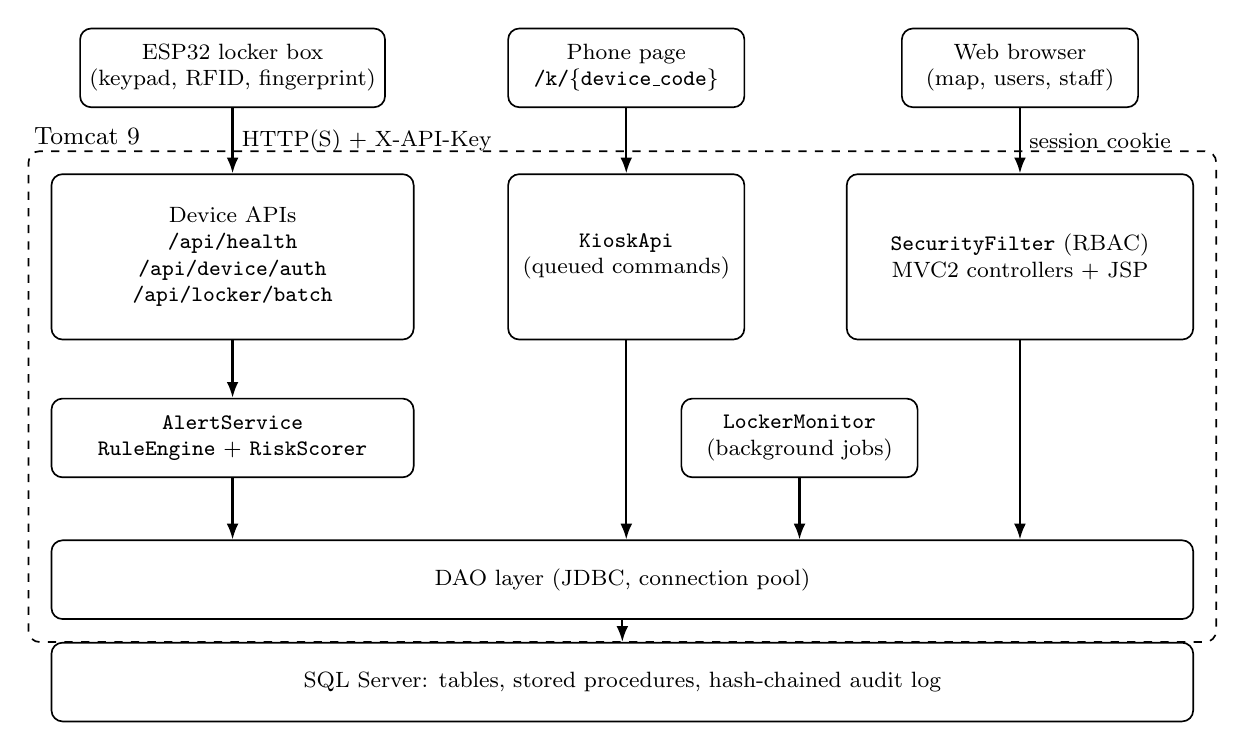
\begin{tikzpicture}[
  box/.style={draw, rounded corners, align=center, minimum height=1.0cm, minimum width=3.0cm, font=\footnotesize},
  tall/.style={box, minimum height=2.1cm},
  arr/.style={-{Latex[length=2mm]}, thick},
  lbl/.style={font=\footnotesize, align=left, inner sep=3pt}]
  \node[box] (esp)   at (0,4.0)  {ESP32 locker box\\(keypad, RFID, fingerprint)};
  \node[box] (phone) at (5,4.0)  {Phone page\\\texttt{/k/\{device\_code\}}};
  \node[box] (web)   at (10,4.0) {Web browser\\(map, users, staff)};
  \node[tall, minimum width=4.6cm] (devapi) at (0,1.6)  {Device APIs\\\texttt{/api/health}\\\texttt{/api/device/auth}\\\texttt{/api/locker/batch}};
  \node[tall, minimum width=3.0cm] (kiosk)  at (5,1.6)  {\texttt{KioskApi}\\(queued commands)};
  \node[tall, minimum width=4.4cm] (ctrl)   at (10,1.6) {\texttt{SecurityFilter} (RBAC)\\MVC2 controllers + JSP};
  \node[box, minimum width=4.6cm] (svc) at (0,-0.7)   {\texttt{AlertService}\\\texttt{RuleEngine} + \texttt{RiskScorer}};
  \node[box, minimum width=3.0cm] (mon) at (7.2,-0.7) {\texttt{LockerMonitor}\\(background jobs)};
  \node[box, minimum width=14.5cm] (dao) at (4.95,-2.5) {DAO layer (JDBC, connection pool)};
  \node[box, minimum width=14.5cm] (db)  at (4.95,-3.8) {SQL Server: tables, stored procedures, hash-chained audit log};
  \draw[arr] (esp)   -- node[lbl, right] {HTTP(S) + X-API-Key} (devapi);
  \draw[arr] (phone) -- (kiosk);
  \draw[arr] (web)   -- node[lbl, right] {session cookie} (ctrl);
  \draw[arr] (devapi) -- (svc);
  \draw[arr] (svc)   -- (svc |- dao.north);
  \draw[arr] (kiosk) -- (kiosk |- dao.north);
  \draw[arr] (ctrl)  -- (ctrl |- dao.north);
  \draw[arr] (mon)   -- (mon |- dao.north);
  \draw[arr] (dao)   -- (db);
  \node[draw, dashed, rounded corners, fit=(devapi)(kiosk)(ctrl)(svc)(mon)(dao), inner sep=8pt,
        label={[font=\small, anchor=south west, inner sep=2pt]north west:Tomcat 9}] {};
\end{tikzpicture}
\caption{System architecture of SmartLocker.}
\label{fig:arch}
\end{figure}

Fig.~\ref{fig:workflow} gives the end-to-end workflow. Credentials and telemetry are captured at the box and forwarded
to the server, which takes the access decision and runs the detector; every outcome is stored as a booking change, an
alert or an audit entry and can then be reviewed by staff or by the user.

\begin{figure}[!htbp]
\centering
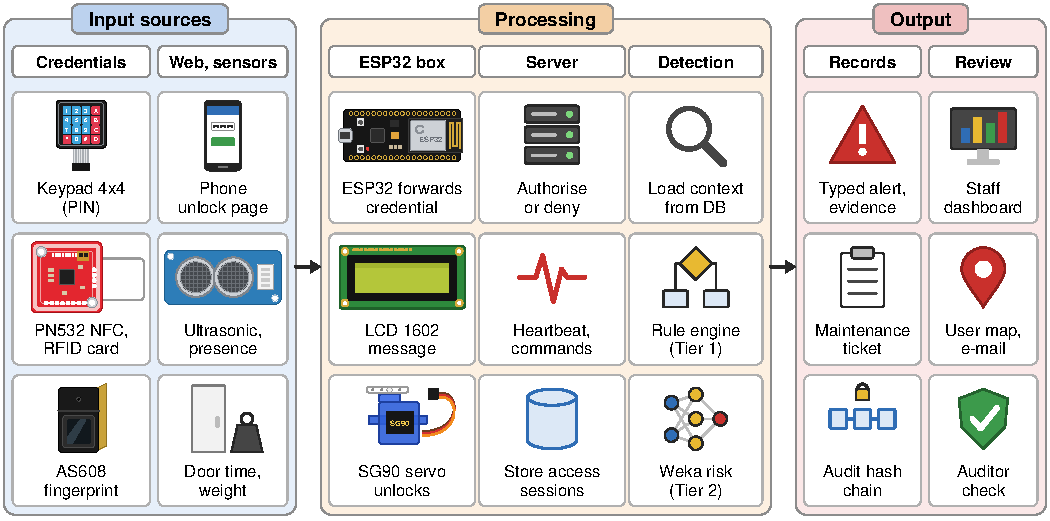
\includegraphics[width=\linewidth]{images/workflow.pdf}
\caption{Workflow of the system. The hardware parts are drawn after those of the prototype box; door time and weight
come from the device simulator, because the box has no door sensor or load cell yet.}
\label{fig:workflow}
\end{figure}

\subsection{Roles}

Access to the web application is governed by role-based access control (RBAC) with five roles: \texttt{END\_USER}
(book, pay, open, extend, cancel, top up), \texttt{OPERATOR} (remote open, top-up approval, areas, banks, slots,
plans, cards, bookings), \texttt{TECHNICIAN} (alerts, maintenance, calibration), \texttt{AUDITOR} (read-only access,
audit-chain verification) and \texttt{ADMIN} (everything, including roles and permissions). Visitors may browse the map
without an account; every other page and every write request requires a session, and the box authenticates with its
own key.

\subsection{Data Model}

Lockers are organised in three levels: an \emph{area} is a pin on the map (Leaflet, or Mapbox GL when a token is
configured), a \emph{bank} is a column of lockers controlled by one device, and a \emph{slot} has size S
($20\times20\times20$~cm), M ($40\times40\times40$~cm) or L ($60\times60\times60$~cm). A booking is a row of
\texttt{Deposit} linking a user, a slot, a plan and optionally a card, and filtered unique indexes reject a second open
booking for the same slot or user. Access sessions are append-only (a trigger blocks updates and deletions), alerts
keep their evidence rows, and remote commands record when they were issued, sent and completed.

\subsection{Hardware}

The locker box is built around an ESP32 development board (Table~\ref{tab:hw} and Fig.~\ref{fig:block}). A 4$\times$4
keypad reads PINs and menu keys, a PN532 NFC reader reads RFID cards, an AS608 optical sensor reads fingerprints, a
16$\times$2 I$^2$C LCD displays messages, and two servos drive the bolt and the door. An SRF05 ultrasonic sensor
detects a person in front of the box and is used only to switch on the LCD backlight. The box sends a heartbeat every
3~s and executes the commands contained in the reply.

\begin{table}[!htbp]
\renewcommand{\arraystretch}{1.1}
\centering
\small
\caption{Hardware Components of the Locker Box}
\label{tab:hw}
\begin{tabular}{l l l}
\hline
Component & Function & ESP32 pins \\
\hline
ESP32 Dev Module & Controller, Wi-Fi, HTTP(S) client & -- \\
PN532 & RFID card reader (I$^2$C, 0x24) & SDA 21, SCL 22 (shared with LCD) \\
AS608 & Fingerprint sensor (UART) & TX$\rightarrow$35, RX 15 \\
LCD 1602 I$^2$C & User messages & SDA 21, SCL 22 \\
Keypad 4$\times$4 & PIN and menu input & Rows 13, 14, 25, 26; columns 33, 19, 23, 27 \\
Servo (bolt / door) & Locks the slot / opens the door & 32 / 2 \\
SRF05 & Presence detection (backlight) & TRIG 5, ECHO 18 \\
\hline
\end{tabular}
\end{table}

\begin{figure}[!htbp]
\centering
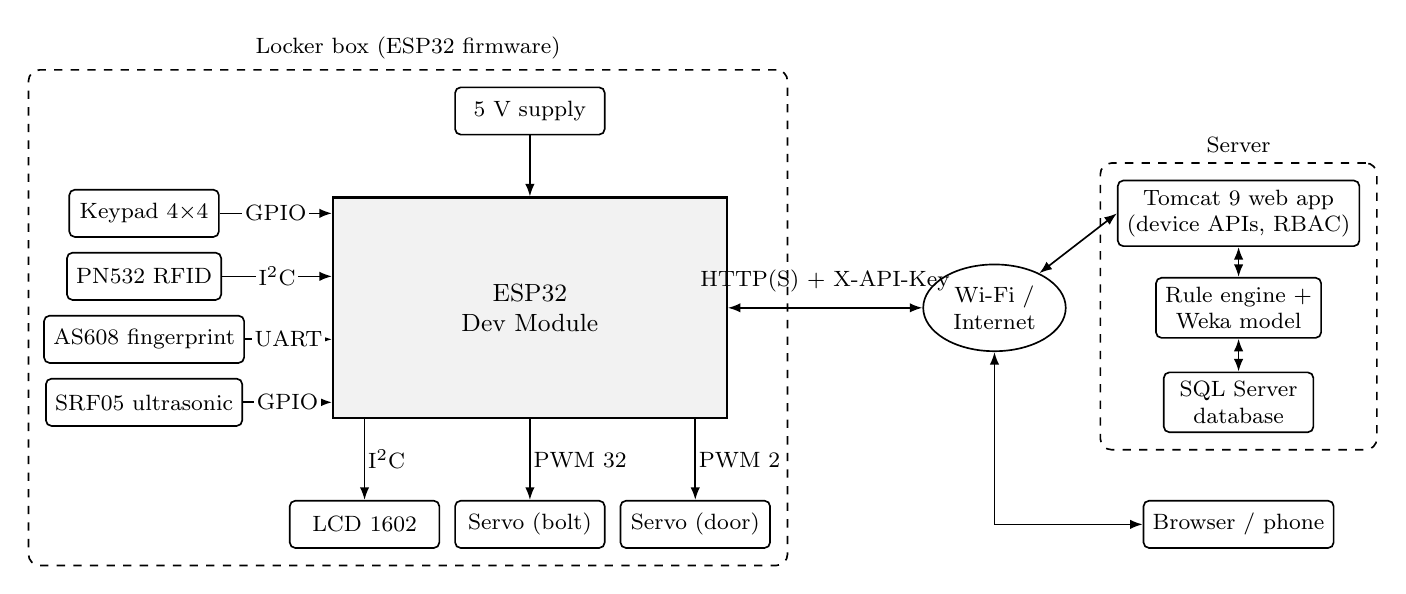
\begin{tikzpicture}[
  b/.style={draw, rounded corners=2pt, font=\footnotesize, align=center, minimum width=1.9cm, minimum height=0.6cm},
  arr/.style={-{Latex[length=1.6mm]}},
  dbl/.style={{Latex[length=1.6mm]}-{Latex[length=1.6mm]}},
  bus/.style={font=\footnotesize, fill=white, inner sep=1pt}]
  \node[draw, thick, fill=gray!10, minimum width=5.0cm, minimum height=2.8cm, font=\small, align=center] (esp) at (0,0) {ESP32\\Dev Module};
  \node[b] (kp)  at (-4.9,1.2)  {Keypad 4$\times$4};
  \node[b] (rf)  at (-4.9,0.4)  {PN532 RFID};
  \node[b] (fp)  at (-4.9,-0.4) {AS608 fingerprint};
  \node[b] (us)  at (-4.9,-1.2) {SRF05 ultrasonic};
  \node[b] (pw)  at (0,2.5)     {5~V supply};
  \node[b] (lcd) at (-2.1,-2.75) {LCD 1602};
  \node[b] (sb)  at (0,-2.75)    {Servo (bolt)};
  \node[b] (sd)  at (2.1,-2.75)  {Servo (door)};
  \draw[arr] (kp.east) -- node[bus] {GPIO}    (kp.east -| esp.west);
  \draw[arr] (rf.east) -- node[bus] {I$^2$C}  (rf.east -| esp.west);
  \draw[arr] (fp.east) -- node[bus] {UART}    (fp.east -| esp.west);
  \draw[arr] (us.east) -- node[bus] {GPIO}    (us.east -| esp.west);
  % straight vertical wires: nothing crosses
  \draw[arr] (pw.south) -- (esp.north);
  \draw[arr] (lcd |- esp.south) -- node[bus, right] {I$^2$C}  (lcd.north);
  \draw[arr] (sb |- esp.south)  -- node[bus, right] {PWM 32} (sb.north);
  \draw[arr] (sd |- esp.south)  -- node[bus, right] {PWM 2}  (sd.north);
  \node[draw, dashed, rounded corners, fit=(kp)(us)(pw)(lcd)(sd)(esp), inner sep=6pt,
        label={[font=\footnotesize]north:Locker box (ESP32 firmware)}] {};
  \node[draw, ellipse, font=\footnotesize, align=center] (net) at (5.9,0) {Wi-Fi /\\Internet};
  \node[b] (tc) at (9.0,1.2)  {Tomcat 9 web app\\(device APIs, RBAC)};
  \node[b] (ml) at (9.0,0)    {Rule engine +\\Weka model};
  \node[b] (db) at (9.0,-1.2) {SQL Server\\database};
  \node[b] (cl) at (9.0,-2.75) {Browser / phone};
  \node[draw, dashed, rounded corners, fit=(tc)(ml)(db), inner sep=6pt,
        label={[font=\footnotesize]north:Server}] {};
  \draw[dbl] (esp.east) -- node[font=\footnotesize, above=2pt] {HTTP(S) + X-API-Key} (net);
  \draw[dbl] (net) -- (tc.west);
  \draw[dbl] (tc) -- (ml);
  \draw[dbl] (ml) -- (db);
  \draw[dbl] (cl.west) -| (net.south);
\end{tikzpicture}
\caption{Block diagram of the prototype box and the server it reaches over Wi-Fi.}
\label{fig:block}
\end{figure}

\subsection{Device Protocol}

Each box holds a secret API key; the database stores only its SHA-256 hash, and the server derives the device
identity from the key, never from the request body. Three endpoints carry the protocol (two more enroll cards and
fingerprints):
\begin{itemize}
  \item \texttt{POST /api/health}: heartbeat every 3~s, whose reply carries pending commands (remote
        \texttt{UNLOCK}, fingerprint deletion) and the blocked card UIDs.
  \item \texttt{POST /api/device/auth}: a PIN, card UID or fingerprint slot with an \emph{intent} (\texttt{ASK},
        \texttt{OPEN}, \texttt{CHECKOUT}), answered by \texttt{UNLOCK}, \texttt{CHOOSE}, \texttt{CONFIRM\_EMAIL} or
        \texttt{DENY} with a reason and the attempts left.
  \item \texttt{POST /api/locker/batch}: buffered access sessions with a per-device sequence number, so a session sent
        again after an outage is stored once.
\end{itemize}
The current firmware does not upload sessions yet, so the batch endpoint is exercised by a device simulator
(Section~VI). A box may control several banks; the \texttt{physical} flag of \texttt{UNLOCK} moves the servo only for
the wired slot. Because a lost card can be used by anyone, a card scan is confirmed by its owner when the server can
send e-mail: the box receives \texttt{CONFIRM\_EMAIL}, and the server releases a held \texttt{UNLOCK} (valid for
5~minutes) after a POST on a single-use link, stored only as a hash, or after a confirmation on the map. A card
presented at the wrong box is refused with \texttt{WRONG\_PLACE}, which names the correct bank. Fig.~\ref{fig:seq}
shows an opening at the box and a remote or phone open, which the box receives with its next heartbeat and reports
back as a session carrying the command identifier.

\begin{figure}[!htbp]
\centering
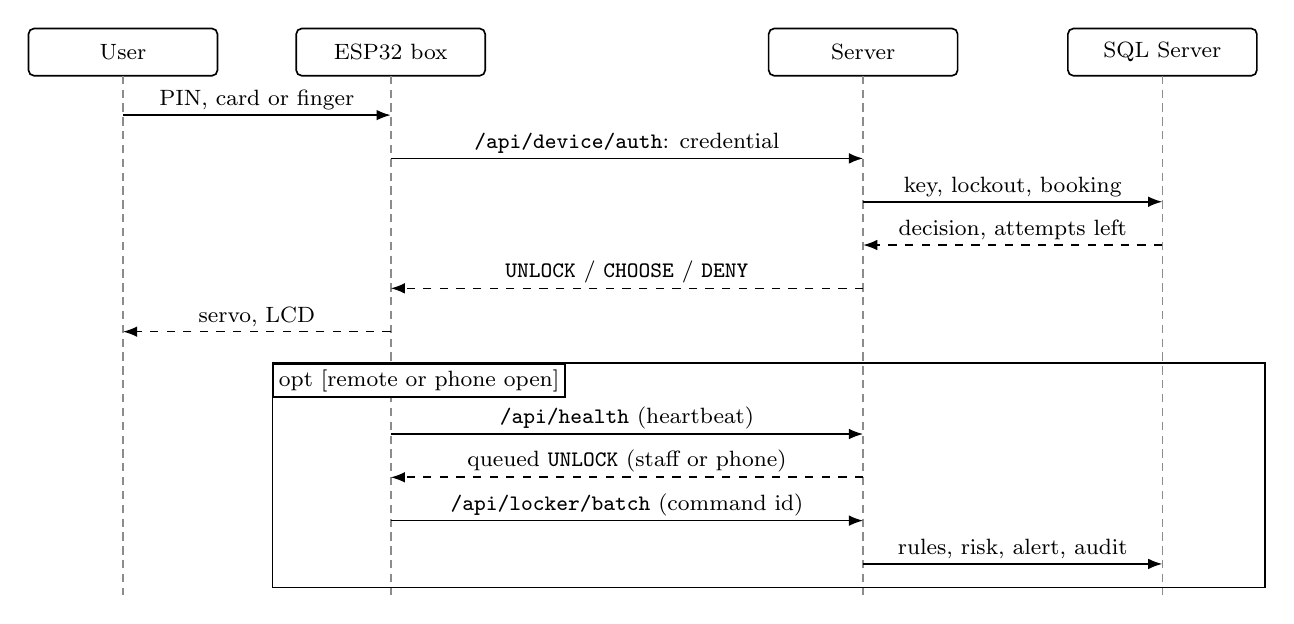
\begin{tikzpicture}[
  head/.style={draw, rounded corners=2pt, font=\footnotesize, minimum width=2.4cm, minimum height=0.6cm},
  msg/.style={-{Latex[length=1.8mm]}},
  ret/.style={-{Latex[length=1.8mm]}, dashed},
  t/.style={font=\footnotesize, above, inner sep=1.5pt}]
  \foreach \x/\n in {0/User, 3.4/ESP32 box, 9.4/Server, 13.2/SQL Server} {
    \node[head] at (\x,0) {\n};
    \draw[densely dashed, black!45] (\x,-0.3) -- (\x,-6.9);
  }
  % opening at the box
  \draw[msg] (0,-0.8)   -- node[t] {PIN, card or finger} (3.4,-0.8);
  \draw[msg] (3.4,-1.35) -- node[t] {\texttt{/api/device/auth}: credential} (9.4,-1.35);
  \draw[msg] (9.4,-1.9) -- node[t] {key, lockout, booking} (13.2,-1.9);
  \draw[ret] (13.2,-2.45) -- node[t] {decision, attempts left} (9.4,-2.45);
  \draw[ret] (9.4,-3.0) -- node[t] {\texttt{UNLOCK} / \texttt{CHOOSE} / \texttt{DENY}} (3.4,-3.0);
  \draw[ret] (3.4,-3.55) -- node[t] {servo, LCD} (0,-3.55);
  % remote or phone open (UML opt fragment)
  \draw (1.9,-3.95) rectangle (14.5,-6.8);
  \node[draw, fill=white, font=\footnotesize, anchor=north west, inner sep=2pt] at (1.9,-3.95) {opt [remote or phone open]};
  \draw[msg] (3.4,-4.85) -- node[t] {\texttt{/api/health} (heartbeat)} (9.4,-4.85);
  \draw[ret] (9.4,-5.4) -- node[t] {queued \texttt{UNLOCK} (staff or phone)} (3.4,-5.4);
  \draw[msg] (3.4,-5.95) -- node[t] {\texttt{/api/locker/batch} (command id)} (9.4,-5.95);
  \draw[msg] (9.4,-6.5) -- node[t] {rules, risk, alert, audit} (13.2,-6.5);
\end{tikzpicture}
\caption{Sequence diagram of the device protocol: an opening at the box (top) and a remote or phone open (UML
\emph{opt} fragment, bottom). Solid arrows are requests, dashed arrows are replies.}
\label{fig:seq}
\end{figure}

\subsection{Booking Lifecycle}

The states of a slot are shown in Fig.~\ref{fig:state}. A reservation charges the wallet and holds the slot for
15~minutes; cancelling within 5~minutes refunds 100\%, later during the hold 50\%, and a no-show nothing, while three
no-shows within 7~days block new bookings for a while. The first authentication at the box is a \texttt{CHECK\_IN},
which starts the due time; later ones offer ``A: open / B: return'', where A keeps the rental (\texttt{ACCESS}) and B
ends it (\texttt{PICKUP}). A booking can be extended three times. An overdue booking is never released, since the
belongings are still inside: after the grace period the slot is \emph{locked}, every late hour costs 150\% of the
hourly rate, the box refuses to open (\texttt{OVERDUE\_UNPAID}) until the debt is paid, and after 48~hours an
\texttt{OVERDUE\_ESCALATED} alert goes to staff.

\begin{figure}[!htbp]
\centering
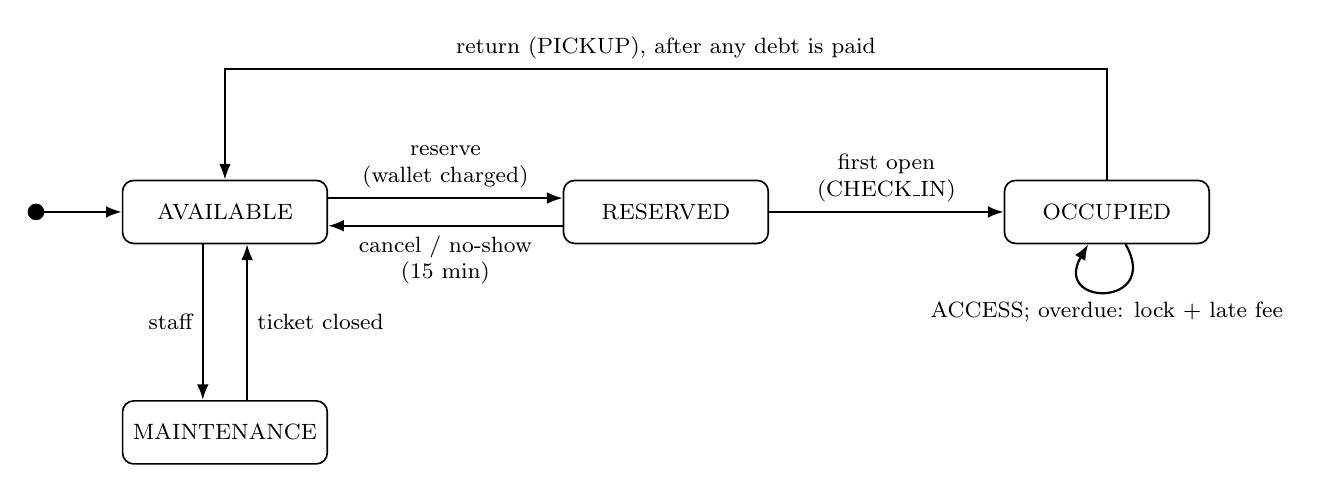
\begin{tikzpicture}[
  st/.style={draw, rounded corners, minimum width=2.6cm, minimum height=0.8cm, font=\footnotesize},
  arr/.style={-{Latex[length=2mm]}, thick},
  lbl/.style={font=\footnotesize, align=center}]
  \node[st] (av)  at (0,0)    {AVAILABLE};
  \node[st] (re)  at (5.6,0)  {RESERVED};
  \node[st] (oc)  at (11.2,0) {OCCUPIED};
  \node[st] (mt)  at (0,-2.8) {MAINTENANCE};
  \fill (-2.4,0) circle (3pt);
  \draw[arr] (-2.3,0) -- (av);
  % two parallel arrows, labels outside them
  \draw[arr] ([yshift=5pt]av.east) -- node[lbl, above] {reserve\\(wallet charged)} ([yshift=5pt]re.west);
  \draw[arr] ([yshift=-5pt]re.west) -- node[lbl, below] {cancel / no-show\\(15 min)} ([yshift=-5pt]av.east);
  \draw[arr] (re) -- node[lbl, above] {first open\\(CHECK\_IN)} (oc);
  % the return runs above every label
  \draw[arr] (oc.north) -- ++(0,1.4) -| node[lbl, above, pos=0.25] {return (PICKUP), after any debt is paid} (av.north);
  \draw[arr] (oc) to[out=-60, in=-120, looseness=5] node[lbl, below] {ACCESS; overdue: lock + late fee} (oc);
  \draw[arr] ([xshift=-8pt]av.south) -- node[lbl, left] {staff} ([xshift=-8pt]mt.north);
  \draw[arr] ([xshift=8pt]mt.north) -- node[lbl, right] {ticket closed} ([xshift=8pt]av.south);
\end{tikzpicture}
\caption{Slot state diagram (the filled dot marks the initial state). An overdue booking stays ACTIVE and its slot
stays OCCUPIED.}
\label{fig:state}
\end{figure}

\section{Anomalous Access Detection}

\subsection{Access Sessions and Context}

Each opening of a slot produces an \emph{access session} described by five features, uploaded through
\texttt{/api/locker/batch}: the door time (how long the door stayed open, in seconds), the weight change inside the
slot (in grams), the number of unlock events, whether a valid RFID card was read, and the stay time (how long the items
remained in the slot, in minutes). A session also records its open source (local, remote or phone), the card UID and,
for a remote open, the identifier of the command. Telemetry alone does not reveal \emph{who} opened the slot, so before
deciding the server loads the context of the session from the database: the status and owner of the card, the owner of
the active booking, whether the remote command was actually issued and is still unused, the stay allowed by the plan,
the valid range of each sensor, the validity of the weight calibration, and the offset between the device clock and
the server clock.

\subsection{Tier 1: Priority-Ordered Rule Engine}

The rules of Table~\ref{tab:rules} are evaluated in a fixed order and the first matching rule determines the label.
The order is essential: readings from a faulty sensor must not be reported as a break-in, and a legitimate remote open
by staff must not be reported as a forced opening. The valid sensor ranges (door 0--3600~s, weight $-200$ to
20\,000~g, stay 0--10\,080~min) are stored in the database, so they can be adjusted without redeploying the
application.

\begin{table}[!htbp]
\renewcommand{\arraystretch}{1.1}
\centering
\small
\caption{Detection Rules in Priority Order}
\label{tab:rules}
\begin{tabular}{c l p{8.4cm} l}
\hline
\# & Label & Condition & Action \\
\hline
1 & SENSOR\_FAULT & door time, weight change or stay time outside the sensor's valid range; door open longer than the whole stay; device clock more than 300~s ahead of the server; weight calibration expired & Alert, ticket, no ML \\
2 & STAFF\_OPEN & remote or phone open with a valid, unused command for this slot, issued at most 30~min before the session (a box clock up to 60~s behind is tolerated) & Command done, no alert \\
2' & SUSPECTED\_SPOOF & remote or phone open without a valid command (never issued, or already used) & Alert \\
3 & LOST\_CARD\_USED & the card is not active (reported lost or blocked) & Alert \\
4 & FORCED\_OPEN & the door opened although no valid card was read & Alert \\
5 & WRONG\_USER & a valid card whose owner is not the owner of the booking & Alert \\
6 & SUSPECTED\_SPOOF & the weight changed by more than 50~g while the door reported ``never opened'' & Alert \\
7 & ITEM\_LEFT & the weight in the slot grew by more than 50~g (items left after pick-up) & Alert \\
8 & OVERDUE & stay time longer than the plan allows & Alert \\
-- & NORMAL & no rule matched & Tier 2 \\
\hline
\end{tabular}
\end{table}

\subsection{Tier 2: Machine-Learning Risk Score}

Let $\mathbf{x}_s = (d, w, u, v, t)$ denote the five features of a session $s$ (door time, weight change, unlocks,
valid card and stay time). A classifier trained offline on labelled sessions estimates the probability that $s$ is
normal, and the \emph{risk score} is defined as
\begin{equation}
r(s) = 1 - P\left(y = \text{NORMAL} \mid \mathbf{x}_s\right).
\label{eq:risk}
\end{equation}
The training tool compares four classifiers (Section~VI) and deploys the six-class model with the highest weighted F1,
which is currently IBk ($k=5$); for a hand-made session with normal-looking telemetry it yields $r = 0.20$. Let
$\ell(s)$ be the label of the first rule of Table~\ref{tab:rules} that matches $s$. The alert raised for $s$ is then
\begin{equation}
A(s) =
\begin{cases}
\ell(s), & \ell(s) \neq \text{NORMAL},\\
\text{ML\_ANOMALY}, & \ell(s) = \text{NORMAL} \text{ and } r(s) \geq \tau,\\
\text{none}, & \text{otherwise},
\end{cases}
\label{eq:alert}
\end{equation}
with the threshold $\tau = 0.80$; when a rule matches, $r(s)$ is stored with its alert as evidence. Without a
deployed model the risk is zero, and it is never computed for SENSOR\_FAULT or STAFF\_OPEN. A STAFF\_OPEN marks its
command as done through a conditional update, so of two sessions carrying the same command only one is a staff open and
the other becomes SUSPECTED\_SPOOF. A SENSOR\_FAULT also takes the slot out of service and opens a maintenance ticket
(one per device), and commands and alerts are written to the audit chain. Fig.~\ref{fig:flow} summarises the decision
flow for one session.

\begin{figure}[!htbp]
\centering
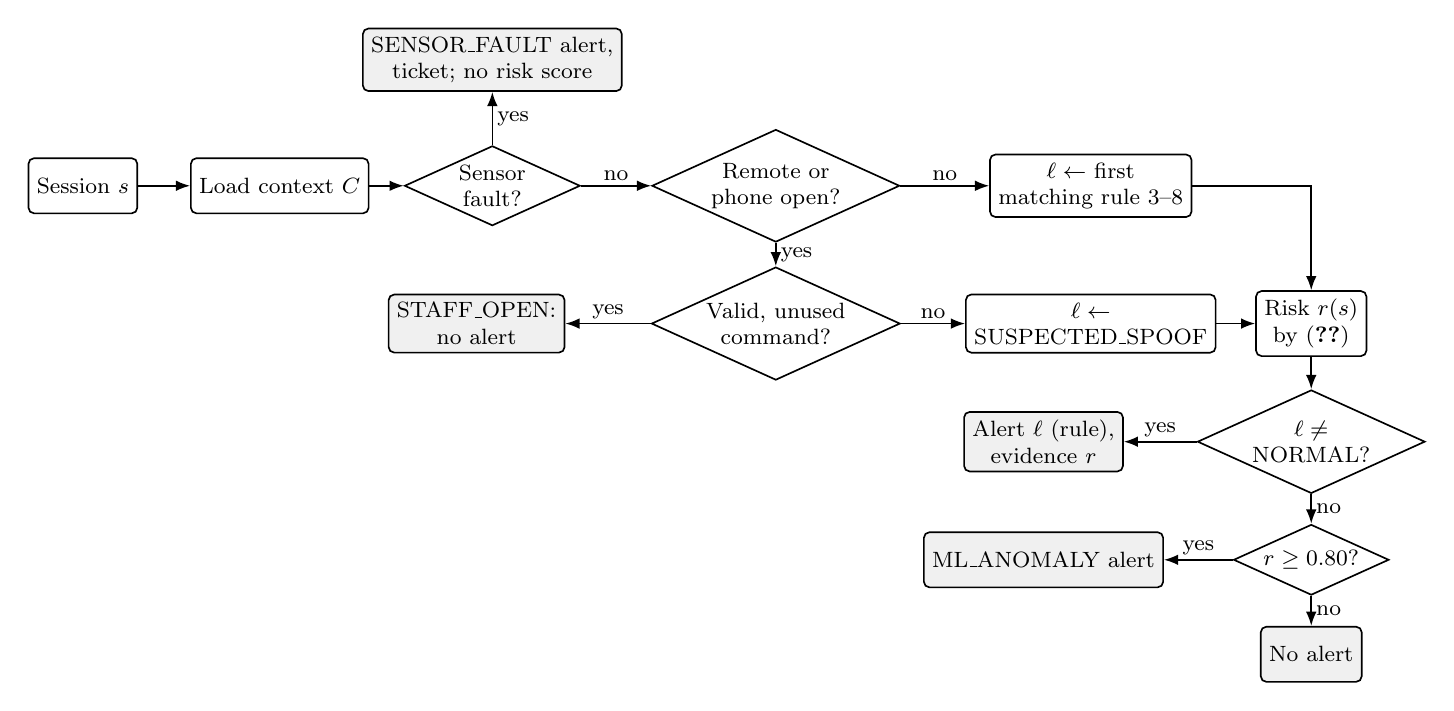
\begin{tikzpicture}[
  proc/.style={draw, rounded corners=2pt, font=\footnotesize, align=center, minimum height=0.7cm, inner sep=3pt},
  term/.style={proc, fill=gray!12},
  dec/.style={draw, diamond, aspect=2.2, font=\footnotesize, align=center, inner sep=1pt},
  arr/.style={-{Latex[length=1.8mm]}},
  yes/.style={font=\footnotesize, inner sep=1.5pt},
  no/.style={font=\footnotesize, inner sep=1.5pt}]
  % top row: input, context, the two first decisions and the rules 3-8
  \node[proc] (in)   at (0,0)      {Session $s$};
  \node[proc] (ctx)  at (2.5,0)    {Load context $C$};
  \node[dec]  (sf)   at (5.2,0)    {Sensor\\fault?};
  \node[dec]  (rem)  at (8.8,0)    {Remote or\\phone open?};
  \node[proc] (rul)  at (12.8,0)   {$\ell \leftarrow$ first\\matching rule 3--8};
  \node[term] (flt)  at (5.2,1.6) {SENSOR\_FAULT alert,\\ticket; no risk score};
  % second row: remote and phone opens, then the merge into the risk score
  \node[dec]  (cmd)  at (8.8,-1.75)  {Valid, unused\\command?};
  \node[term] (stf)  at (5.0,-1.75)  {STAFF\_OPEN:\\no alert};
  \node[proc] (spf)  at (12.8,-1.75) {$\ell \leftarrow$\\SUSPECTED\_SPOOF};
  \node[proc] (rsk)  at (15.6,-1.75) {Risk $r(s)$\\by (\ref{eq:risk})};
  % right column: the alert decision of (2)
  \node[dec]  (lab)  at (15.6,-3.25) {$\ell \neq$\\NORMAL?};
  \node[term] (ar)   at (12.2,-3.25) {Alert $\ell$ (rule),\\evidence $r$};
  \node[dec]  (thr)  at (15.6,-4.75) {$r \geq 0.80$?};
  \node[term] (am)   at (12.2,-4.75) {ML\_ANOMALY alert};
  \node[term] (non)  at (15.6,-5.95) {No alert};
  \draw[arr] (in) -- (ctx);
  \draw[arr] (ctx) -- (sf);
  \draw[arr] (sf) -- node[yes, right] {yes} (flt);
  \draw[arr] (sf) -- node[no, above] {no} (rem);
  \draw[arr] (rem) -- node[no, above] {no} (rul);
  \draw[arr] (rem) -- node[yes, right] {yes} (cmd);
  \draw[arr] (cmd) -- node[yes, above] {yes} (stf);
  \draw[arr] (cmd) -- node[no, above] {no} (spf);
  \draw[arr] (rul.east) -| (rsk.north);
  \draw[arr] (spf) -- (rsk);
  \draw[arr] (rsk) -- (lab);
  \draw[arr] (lab) -- node[yes, above] {yes} (ar);
  \draw[arr] (lab) -- node[no, right] {no} (thr);
  \draw[arr] (thr) -- node[yes, above] {yes} (am);
  \draw[arr] (thr) -- node[no, right] {no} (non);
\end{tikzpicture}
\caption{Decision flow of the two-tier detector for one access session: the rules of Table~\ref{tab:rules} are applied
first, and the risk score of (\ref{eq:risk}) raises an ML\_ANOMALY alert only when no rule matched, as in
(\ref{eq:alert}). Shaded boxes are outcomes.}
\label{fig:flow}
\end{figure}

\subsection{Server-Side Safeguards}

Several abnormal situations are visible from the server state alone.
\begin{itemize}
  \item \textit{Credential guessing.} Every wrong PIN, unknown card or unknown finger counts towards a lockout: five
        wrong guesses within 5~minutes lock the box for 120~s; the phone page has its own counter (five tries,
        2~minutes).
  \item \textit{Silent devices.} A job running every 15~s marks a box without heartbeat for more than 90~s as
        \texttt{OFFLINE}, raises \texttt{DEVICE\_OFFLINE} and stops bookings on its banks.
  \item \textit{Lost cards} are pushed to the box in the blocked list of the next heartbeat (\texttt{CARD\_BLOCKED}).
  \item \textit{Card at the wrong box.} \texttt{WRONG\_PLACE} is logged on the booking the card was meant for, shown
        on the owner's map and e-mailed at most once per 10~minutes; it is not counted as a guess.
  \item \textit{Overdue storage} is locked, charged and escalated after 48~hours with its evidence.
\end{itemize}

\subsection{Tamper-Evident Audit Log}

Every business action and alert is appended to an audit log whose entries store the SHA-256 hash of their fields
(identifier, time, actor, action, object, change) and the hash of the previous entry \cite{haber1991timestamp}. The
last entry is read under an update lock, so concurrent writers cannot fork the chain, and changing or deleting an entry
breaks every later hash. Auditors verify the chain from the web, and a thread re-verifies it every 60~s.

\section{Implementation}

The server is written in Java~8 (about 11\,400 lines in 88 source files) with 21 JSP views and uses Gson,
jBCrypt \cite{provos1999bcrypt} and Weka \cite{hall2009weka}. The interface is in Vietnamese, loads no script from a
content delivery network (Leaflet and Mapbox GL are bundled) and offers light and dark themes; when map tiles cannot be
loaded, the pins are drawn over a plain grid.

\textit{Business rules in the database.} Every rule involving money or time (reservation, refund, extension,
overdue fee, escalation) is a stored procedure. Procedures that read and then modify a row lock it with
\texttt{UPDLOCK, HOLDLOCK} inside the transaction, so a slot cannot be booked twice and an extension cannot be charged
twice. The price of a plan is multiplied by a size factor (S 100\%, M 130\%, L 169\%) and rounded up to 100~VND
(Table~\ref{tab:price}); the late fee is 150\% of the unrounded hourly rate derived from the 2-hour plan, rounded once,
which is why size M pays 4\,900~VND and not 1.5 times 3\,300~VND. Users may also book 1--23 whole hours at the hourly
rate, capped at the day pass, or 1--7 whole days (90\% of the day pass per day for 2--6 days, 80\% for 7 days). All
opening methods cost the same.

\begin{table}[!htbp]
\renewcommand{\arraystretch}{1.1}
\centering
\small
\caption{Prices by Plan and Slot Size (VND)}
\label{tab:price}
\begin{tabular}{l r r r}
\hline
Plan & S & M & L \\
\hline
2 hours & 5\,000 & 6\,500 & 8\,500 \\
4 hours & 9\,000 & 11\,700 & 15\,300 \\
Day pass & 25\,000 & 32\,500 & 42\,300 \\
Hourly rate (extension) & 2\,500 & 3\,300 & 4\,300 \\
Late fee per hour (150\%) & 3\,800 & 4\,900 & 6\,400 \\
\hline
\end{tabular}
\end{table}

\textit{Monitoring.} A background thread (\texttt{LockerMonitor}) rebuilds an in-memory dashboard snapshot every
2~s, so polling dashboards never query the database, and runs the expiry procedures every 15~s; two more threads
re-verify the audit chain every 60~s and send due reminders by e-mail 15~minutes before a booking ends.

\textit{Security.} Passwords are hashed with BCrypt and device keys stored as SHA-256 hashes; the session user is
reloaded on every request, so a locked account is signed out at once; a failed sign-in is logged with the account name
only if that account exists; and all user data is escaped in JSP and JavaScript.

\textit{User interface.} Fig.~\ref{fig:ui} shows the map and a booking as seen by a user, and the dashboard and an
escalated alert as seen by staff.

\begin{figure}[!htbp]
\centering
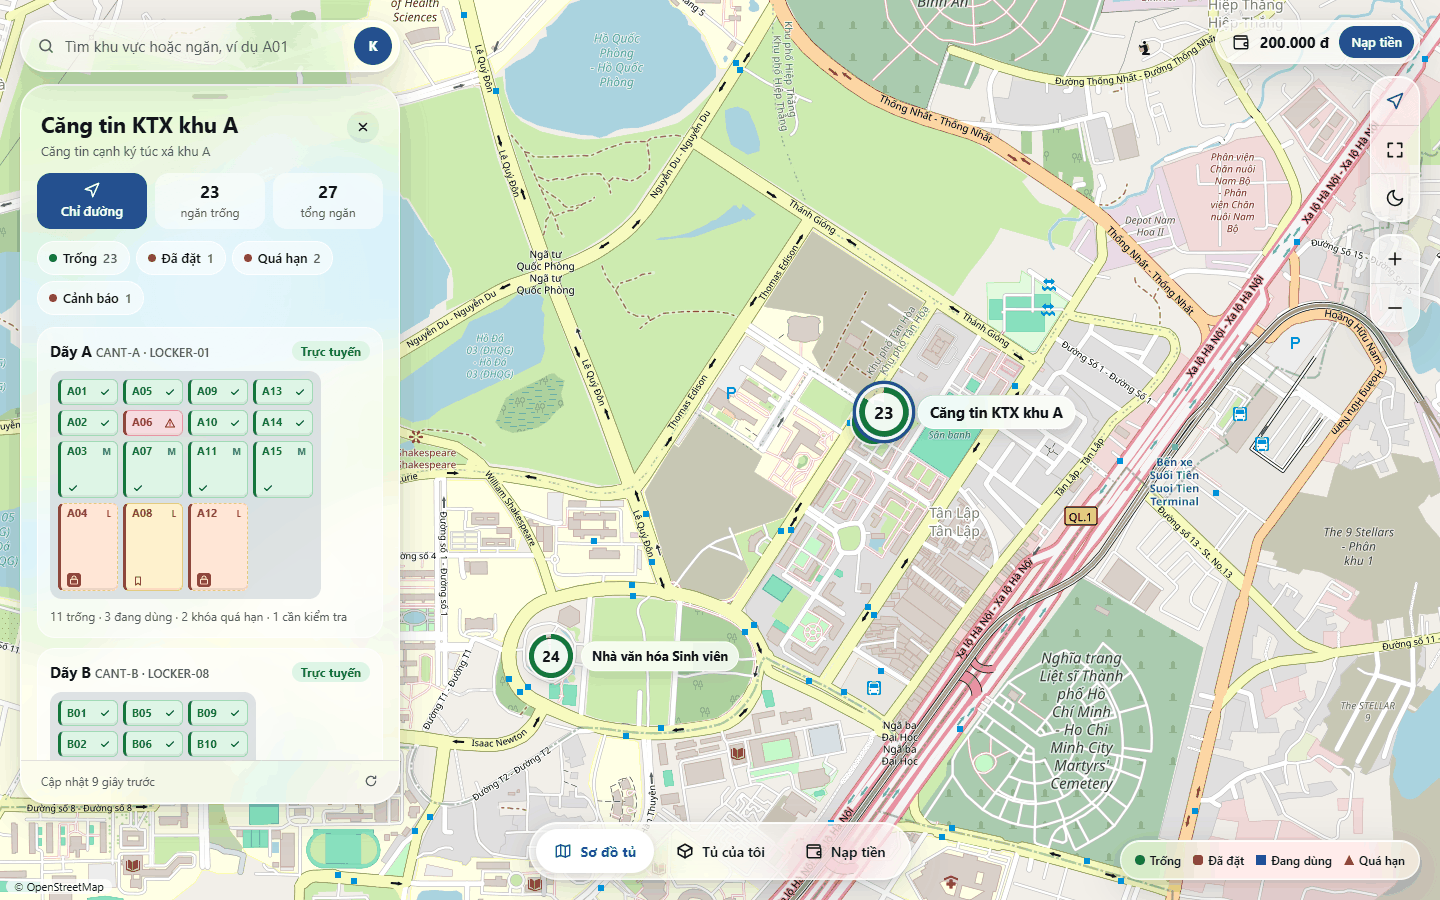
\includegraphics[width=0.38\linewidth]{images/map-area.png}
\hspace{0.04\linewidth}
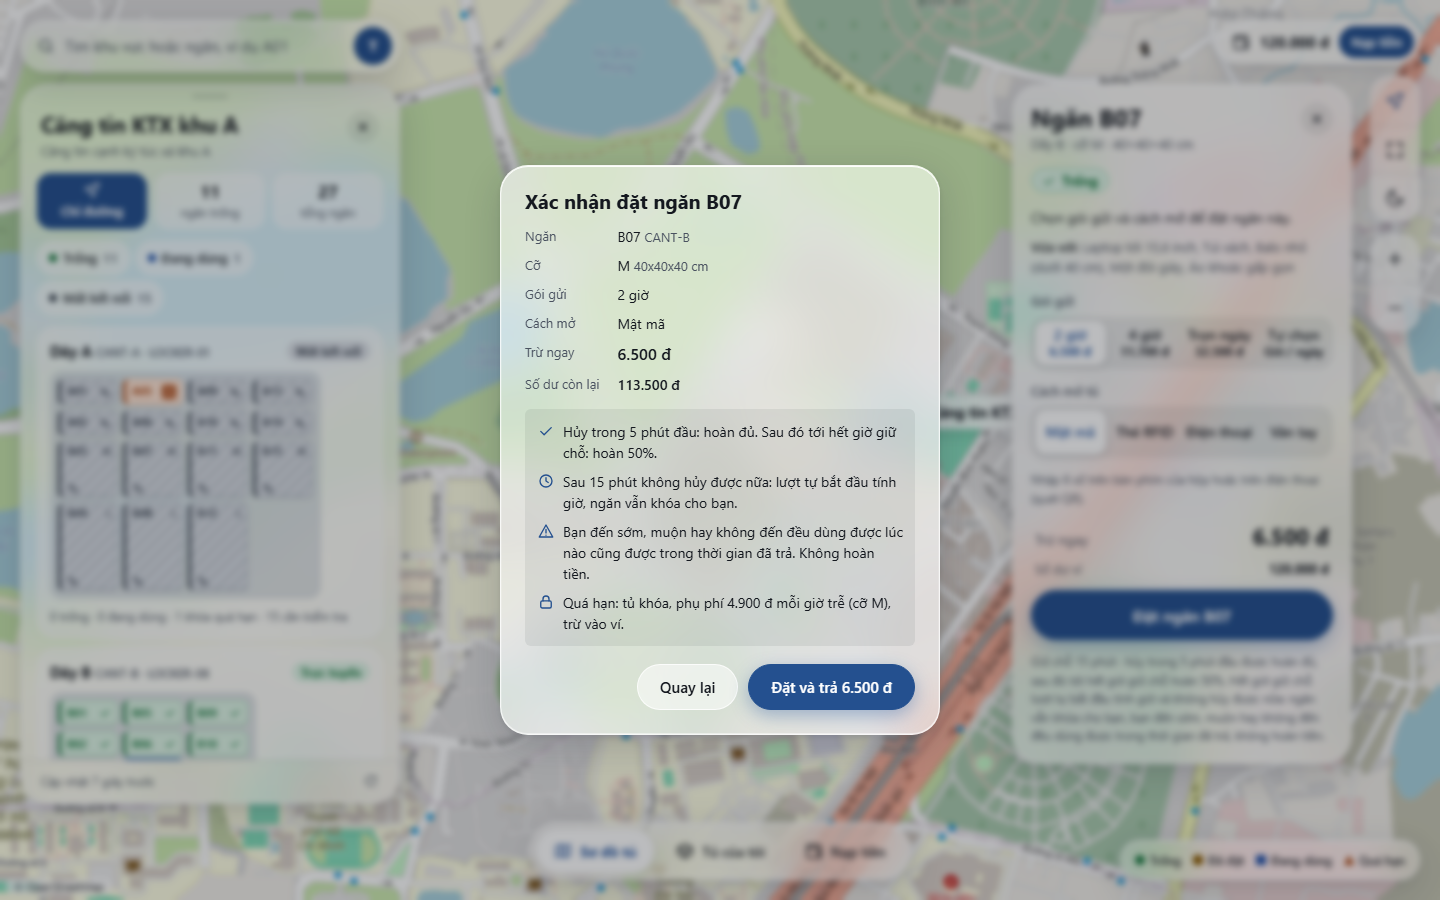
\includegraphics[width=0.38\linewidth]{images/booking-confirm.png}\\[4pt]
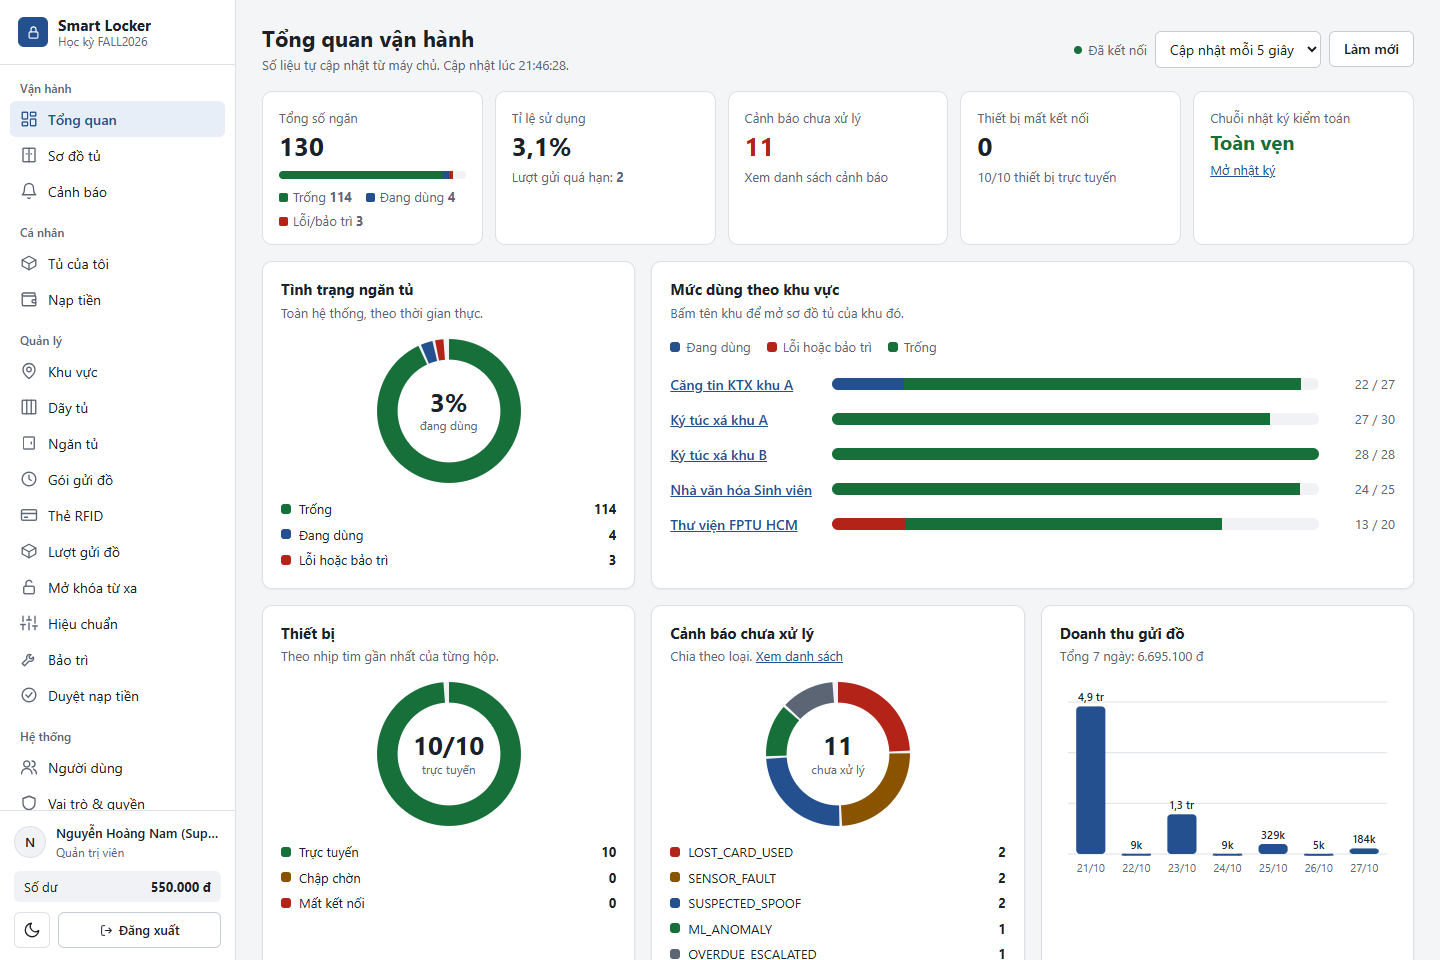
\includegraphics[width=0.38\linewidth]{images/dashboard.png}
\hspace{0.04\linewidth}
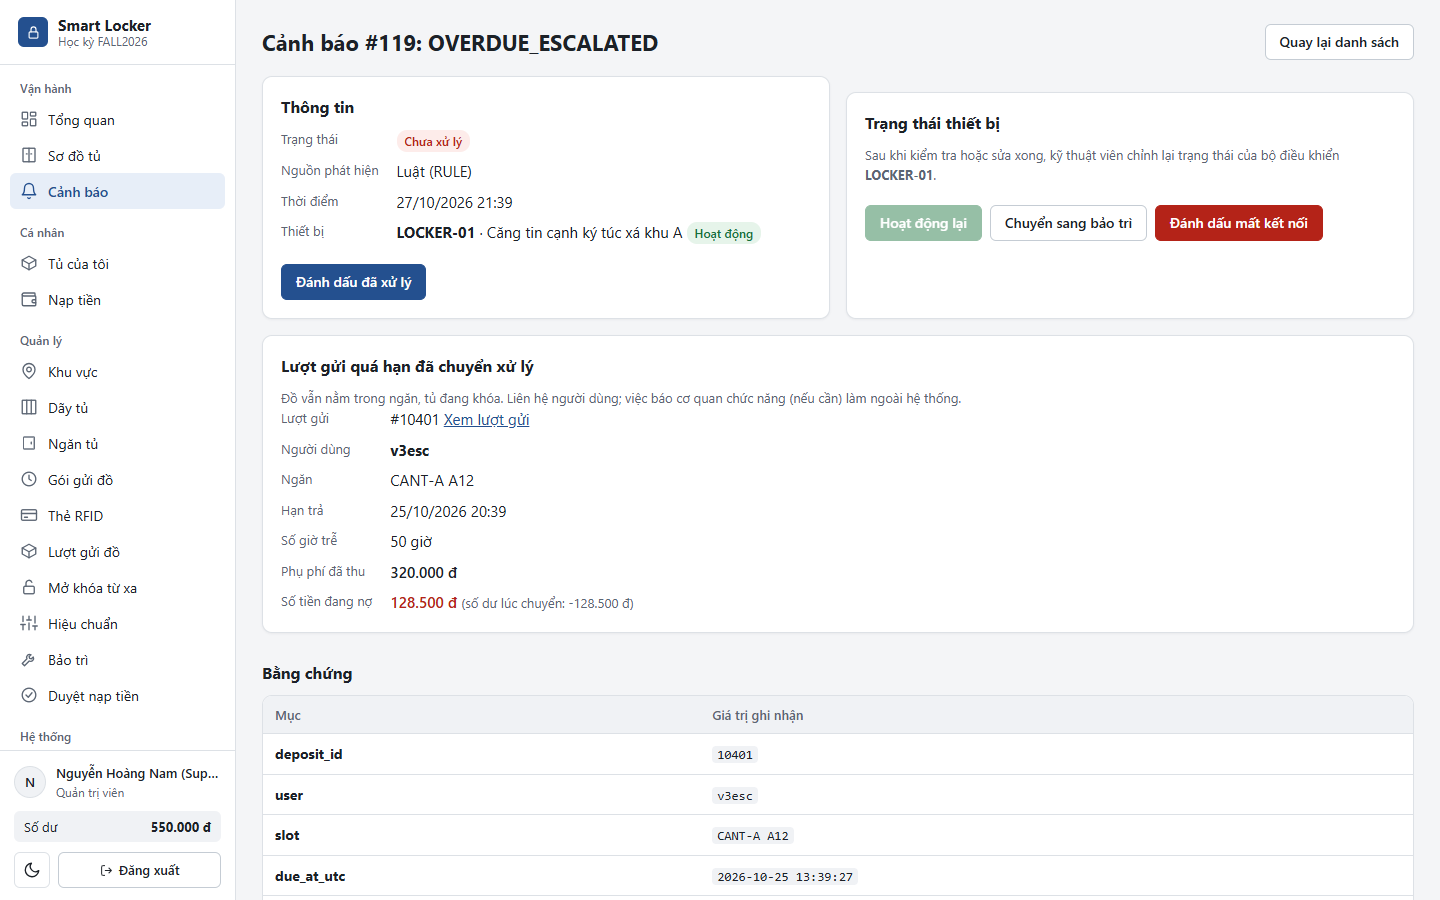
\includegraphics[width=0.38\linewidth]{images/alert-escalated.png}
\caption{User interface (in Vietnamese). Top left: the map with area ``C\u{a}ng tin KTX khu A'', 23 of its 27 slots
free; in bank CANT-A (box LOCKER-01) two slots are locked as overdue and one has an open alert. Top right: the booking
confirmation of slot B07 (bank CANT-B, size M, 2-hour plan, PIN), which takes 6\,500~VND now and states the refund and
late-fee rules. Bottom left: the staff dashboard with 130 slots, 11 open alerts by type, 10 of 10 devices online, the
audit-chain status and the revenue of the last 7 days. Bottom right: alert \#119, \texttt{OVERDUE\_ESCALATED}, for a
booking in slot CANT-A A12 that was 50~hours late (320\,000~VND late fee charged, 128\,500~VND owed), with its evidence.
All devices except LOCKER-01 are demo devices whose heartbeat is simulated by the server.}
\label{fig:ui}
\end{figure}

\section{Evaluation}
\label{sec:ml}

\subsection{Experimental Setup}

\textit{Dataset.} The risk model is trained on 480 labelled telemetry sessions described by the five features of
Section~IV-A and divided into six classes (NORMAL, FORCED\_OPEN, WRONG\_USER, OVERDUE, ITEM\_LEFT and
SUSPECTED\_SPOOF) of 80 sessions each. Because the prototype box has neither a door sensor nor a load cell, the
sessions are synthetic: the database seed script generates them from simple per-class patterns, for example no valid
card, a long door time and several unlock events for a forced opening, or a positive weight change for an item left
behind. Wrong-user sessions are produced by exactly the same formulas as normal ones, since the telemetry of a wrong
user is that of an ordinary visit; the two classes differ only in the row index that the formulas take as input.

\textit{Protocol.} Four Weka classifiers with default parameters were compared: Random Forest \cite{breiman2001rf},
J48 (C4.5) \cite{quinlan1993c45}, Naive Bayes \cite{john1995nb} and IBk with $k = 5$ \cite{aha1991ibl}. Each was
evaluated by stratified 10-fold cross-validation \cite{kohavi1995cv} (seed 42) on the six-class problem and on a binary
NORMAL-versus-ABNORMAL problem, which measures the decision taken by the risk score and is not deployed. Training time
is the median of 11 builds and inference time the mean over $20 \times 480$ predictions after a warm-up, both repeated
in three runs. The experiments ran on an Intel Core i5-11400H laptop (2.7~GHz, 6 cores, 16~GB RAM, 64-bit Windows~11)
with Oracle JDK 1.8.0\_202 and Weka 3.8.6; the server measurements of Section~\ref{sec:latency} used Tomcat 9.0.113 (JDK
1.8.0\_171) and SQL Server 2022 on the same machine.

\subsection{Classification Results}

\begin{table}[!htbp]
\renewcommand{\arraystretch}{1.1}
\centering
\small
\caption{10-Fold Cross-Validation Results (Weighted Averages)}
\label{tab:ml}
\begin{tabular}{l c c c c c c}
\hline
 & \multicolumn{4}{c}{Six classes} & \multicolumn{2}{c}{Binary} \\
Model & Accuracy & Precision & Recall & F1 & Accuracy & F1 \\
\hline
Random Forest & 0.948 & 0.949 & 0.948 & 0.948 & 0.938 & 0.939 \\
J48 (C4.5)    & 0.856 & 0.857 & 0.856 & 0.856 & 0.831 & 0.848 \\
Naive Bayes   & 0.779 & 0.778 & 0.779 & 0.778 & 0.833 & 0.852 \\
IBk ($k=5$)   & 0.977 & 0.978 & 0.977 & 0.977 & 0.975 & 0.975 \\
\hline
\end{tabular}
\end{table}

As Table~\ref{tab:ml} shows, IBk achieves the highest weighted F1 in both settings (0.977 and 0.975), followed by
Random Forest (0.948 and 0.939), while Naive Bayes is the weakest model in the six-class setting (0.778). All four
models are inexpensive enough for online scoring. In the six-class setting, Random Forest trains in about 36--38~ms and
scores a session in 12--15.5~$\mu$s, whereas IBk requires essentially no training (under 1~ms) and scores a session in
15--17~$\mu$s (ranges over the three runs).

\subsection{Discussion}

Per class, the deployed IBk model classifies all 80 FORCED\_OPEN and OVERDUE sessions correctly (F1 1.000), all 80
SUSPECTED\_SPOOF sessions and 79 of 80 ITEM\_LEFT sessions (F1 0.994 each, the remaining ITEM\_LEFT session being
labelled SUSPECTED\_SPOOF), because every abnormal class except WRONG\_USER alters at least one feature in a
characteristic way. The other 10 of its 11 errors involve WRONG\_USER and NORMAL: 7 wrong-user sessions are labelled
NORMAL and 3 normal sessions WRONG\_USER (F1 0.936 and 0.939). Random Forest shows the same pattern (17 and 8 sessions).
This follows from the construction of the data rather than from an empirical observation: a valid card of another
person produces the telemetry of a normal visit, and the residual separation is an artefact of the row index in the
generator. In the binary setting, Naive Bayes classifies every normal session correctly but labels 80 of the 400
abnormal sessions as NORMAL.

The design does not rest on these scores. Wrong-user access is a question of \emph{identity}, answered exactly by
rule~5, which compares the card owner with the booking owner; lost cards and spoofed remote opens are likewise decided
from the card status and the command table. The learned model is only a secondary signal for unusual combinations of
door time, weight and stay time, and its alerts carry the source ML so that operators treat them with caution
\cite{sommer2010outside}.

\subsection{Functional Testing}

The system was tested at three levels.
\begin{itemize}
  \item \textit{Unit and integration tests} (TestNG). Sixty-six tests cover the rule engine (14 tests), the risk
        scorer, pricing in Java and its agreement with SQL, the audit hash chain, the device heartbeat, pick-up and
        bank-assignment rules, password and key hashing, e-mail templates, card confirmation links and box messages;
        all 66 passed and none was skipped.
  \item \textit{API scenarios} (Postman/newman). Eighteen scenarios cover PIN, phone, card and fingerprint access,
        lost cards, wrong keys, bodies and codes, the five-try lockout, no-show, overdue lock, top-up, cancellation,
        escalation, extension and repeated opens. The first run failed one assertion: with two banks that both contain
        a slot A01, a session upload returned HTTP 500 because the slot was looked up by box and slot code only; the
        server now resolves it by bank code or by the command's slot and otherwise rejects the session as
        \texttt{AMBIGUOUS\_SLOT}. Every later run (2~min 27~s on the released build) executed 221 requests and 472
        assertions without a failure.
  \item \textit{Detection scenarios}. A device simulator sends heartbeats, credentials and session uploads signed with
        the key of the real box LOCKER-01, and the database is inspected after each scenario (Table~\ref{tab:scen}).
\end{itemize}

\begin{table}[!htbp]
\renewcommand{\arraystretch}{1.1}
\centering
\small
\caption{Detection Scenarios Replayed through the Device API}
\label{tab:scen}
\begin{tabular}{l p{5.0cm} p{3.0cm} p{5.8cm}}
\hline
Scenario & Input & Expected & Observed \\
\hline
heartbeat & 6 heartbeats 10~s apart, then silence & DEVICE\_OFFLINE in 90--105~s & \texttt{OFFLINE} and alert 104.6~s after the last heartbeat \\
remote    & staff remote open; the box reports it with the command id, then replays it & STAFF\_OPEN; replay SUSPECTED\_SPOOF & no alert, command \texttt{DONE}; replay \texttt{SUSPECTED\_SPOOF} \\
spoof     & remote session with a command id never issued & SUSPECTED\_SPOOF & \texttt{SUSPECTED\_SPOOF} \\
lostcard  & card reported lost, then used at the box & LOST\_CARD\_USED & \texttt{LOST\_CARD\_USED}; card in the blocked list \\
checkin   & reservation, then its PIN sent to \texttt{/api/device/auth} & UNLOCK, CHECK\_IN & booking \texttt{ACTIVE}, slot \texttt{OCCUPIED}, no alert \\
sensor    & weight change of $-5000$~g (range $-200$ to 20\,000~g) & SENSOR\_FAULT & slot \texttt{MAINTENANCE}; existing ticket kept \\
\hline
\end{tabular}
\end{table}

All six scenarios produced the expected label, although two required an adjustment. In the first \emph{remote} run, the
simulator stamped the session in whole seconds, earlier than the command created within the same second, and both
sessions were therefore flagged as spoofed. Since a box clock that lags the server would cause the same false alarm,
the rule now accepts a session stamped up to 60~s before its command, and a rule-engine test covers this window. The
simulator's own \emph{checkin} case sent only a heartbeat, which no longer checks a booking in; the PIN was therefore
sent to \texttt{/api/device/auth}, as the real box does.

\subsection{Server-Side Response Time}
\label{sec:latency}

The real box was offline during these measurements, so Table~\ref{tab:latency} reports the \emph{server processing
time} of the device API only: 30 requests per endpoint were sent with curl from the same laptop after one warm-up
request, which excludes Wi-Fi, credential reading and servo movement. The PIN requests used the valid PIN of an active
booking with intent \texttt{ASK}, which the server answers with the ``A: open / B: return'' choice without modifying
any data.

\begin{table}[!htbp]
\renewcommand{\arraystretch}{1.1}
\centering
\small
\caption{Server-Side Response Time of the Device API (localhost, 30 Requests Each, ms)}
\label{tab:latency}
\begin{tabular}{l c c c c c}
\hline
Request & Mean & Median & p95 & Min & Max \\
\hline
Heartbeat (\texttt{/api/health})                   & 5.9  & 6.0  & 6.8  & 4.6  & 7.3 \\
PIN at the box (\texttt{/api/device/auth})         & 17.0 & 15.7 & 19.0 & 14.1 & 48.0 \\
PIN on the phone page (\texttt{/api/kiosk/unlock}) & 31.1 & 16.2 & 96.0 & 13.4 & 102.7 \\
\hline
\end{tabular}
\end{table}

Every request was answered within about 0.1~s, so the wait at the box is dominated by Wi-Fi, the readers and the
servo; a phone-page open also waits for the next heartbeat (every 3~s). \textit{Lockout:} wrong PINs 1 to 4 were
answered with 4 down to 1 attempts left, the fifth started a 120~s lock that also refused the valid PIN
(\texttt{LOCKED\_OUT}), and the valid PIN was accepted again 125.5~s after the lock started. \textit{Offline
detection:} with a 90~s timeout checked every 15~s, the expected delay is 90--105~s; the heartbeat scenario measured
104.6~s and four earlier offline alerts of the same box took 97--98~s (one more took 110~s because the application was
reloaded).

\textit{End-to-end opening on the real box:} 20 openings from the phone page took 1.67~s on average from sending the PIN
until the door opened. Most of this delay is the wait for the next heartbeat of the box (every 3~s, hence 1.5~s on
average), and the server time reported above is only a small part of it.

\subsection{Limitations}

The evaluation has four main limitations. First, the box has no door sensor or load cell and does not yet upload
sessions, so every session comes from the device simulator or the seed data. Second, the training data are synthetic,
with simple class patterns and shared formulas for wrong-user and normal sessions, so the cross-validation scores are
optimistic; a transfer test on about 100 labelled device sessions is implemented but could not be run. Third, only one
slot has a physical lock, and the other banks belong to demo devices. Fourth, transport security is basic: forms carry
no CSRF token (only the \texttt{SameSite=Lax} cookie), Tomcat serves plain HTTP, HTTPS comes only from a Cloudflare
tunnel, and the firmware does not verify the server certificate (\texttt{setInsecure}).

\section{Conclusion}

This paper presented SmartLocker, a locker rental system with online reservation, size-based pricing, four opening
methods and an ESP32 box that delegates every decision to the server. Anomalous access is detected by a
priority-ordered rule engine over telemetry and server context, backed by a machine-learning risk score for cases that
no rule describes, and completed by a 120~s lockout, offline detection within 90--105~s, overdue locking with 48-hour
escalation and a hash-chained audit log. On 480 synthetic sessions, IBk reached a weighted F1 of 0.977 and Random
Forest 0.948; their errors between wrong-user and normal sessions illustrate, rather than prove, that identity checks
belong in explicit rules. The system passed all 66 tests and 472 API assertions, the six detection scenarios produced
the expected labels, and the server answered device requests in a mean of 6--31~ms per endpoint. Future work will add a
reed switch and a load cell with session upload, collect and label real sessions to train and evaluate the model, time
every opening method end to end, lock several slots physically, and add CSRF tokens and certificate verification on
the box.

\section*{Acknowledgment}

The authors thank FPT University for supporting this course project. During the preparation of this paper, the authors
used the generative AI assistant Claude (Anthropic) to edit and shorten the English text, to check the \LaTeX{}
source, and to draw Fig.~\ref{fig:workflow}, Fig.~\ref{fig:block}, Fig.~\ref{fig:seq} and Fig.~\ref{fig:flow}. The
design, implementation, experiments and all reported measurements are the authors' own; the authors reviewed and edited
every AI-assisted part and take full responsibility for the content of this paper.

\bibliographystyle{IEEEtran}
\bibliography{smartlocker-refs}

\end{document}
